%----------------------------------------------------------------------------------------
% Requisiti
%----------------------------------------------------------------------------------------

\documentclass[10pt]{softeng} % Document font size and equations flushed left

%----------------------------------------------------------------------------------------
%	DOCUMENT INFORMATION
%----------------------------------------------------------------------------------------

\include{current-phase}

\DocumentTitle{Use Case Model} % Document title

\externaldocument[req:]{requirements}
\def\idVERSTOR{REQ\_VERSTOR\_F\_A\_1\,}
\def\shortidVERSTOR{REQ\_F\_1\,}

\def\idSECAUTH{REQ\_SECAUTH\_N\_A\_1\,}
\def\shortidSECAUTH{REQ\_N\_1\,}

\def\idCLIACC{REQ\_CLIACC\_F\_A\_2\,}
\def\shortidCLIACC{REQ\_F\_2\,}

\def\idAPPRCORR{REQ\_APPRCORR\_F\_A\_3\,}
\def\shortidAPPRCORR{REQ\_F\_3\,}

\def\idUSRBID{REQ\_USRBID\_F\_A\_4\,}
\def\shortidUSRBID{REQ\_F\_4\,}

\def\idLOGOP{REQ\_LOGOP\_N\_A\_2\,}
\def\shortidLOGOP{REQ\_N\_2\,}

\def\idCROPVEL{REQ\_CROPVEL\_F\_M\_5\,}
\def\shortidCROPVEL{REQ\_F\_5\,}

\def\idVERTIT{REQ\_VERTIT\_F\_M\_6\,}
\def\shortidVERTIT{REQ\_F\_6\,}

\def\idISCRCORR{REQ\_ISCRCORR\_F\_A\_7\,}
\def\shortidISCRCORR{REQ\_F\_7\,}

\def\idAPPBID{REQ\_APPBID\_F\_A\_8\,}
\def\shortidAPPBID{REQ\_F\_8\,}

\def\idDIPACC{REQ\_DIPACC\_F\_A\_9\,}
\def\shortidDIPACC{REQ\_F\_9\,}

\def\idCREABID{REQ\_CREABID\_F\_A\_10\,}
\def\shortidCREABID{REQ\_F\_10\,}

\def\idDISOPVEL{REQ\_DISOPVEL\_F\_M\_11\,}
\def\shortidDISOPVEL{REQ\_F\_11\,}

\def\idDISPAG{REQ\_DISPAG\_F\_A\_12\,}
\def\shortidDISPAG{REQ\_F\_12\,}

\def\idVERSAL{REQ\_VERSAL\_F\_A\_13\,}
\def\shortidVERSAL{REQ\_F\_13\,}

\def\idPRIVCORR{REQ\_PRIVCORR\_F\_A\_14\,}
\def\shortidPRIVCORR{REQ\_F\_14\,}



%----------------------------------------------------------------------------------------

\begin{document}

\startofdocument{}

\def\iducCROPVEL{UC\_CROPVEL\_1\,}
\def\shortiducCROPVEL{UC\_1\,}
\def\iducDISPAG{UC\_DISPAG\_2\,}
\def\shortiducDISPAG{UC\_2\,}
\def\iducISCRCORR{UC\_ISCRCORR\_3\,}
\def\shortiducISCRCORR{UC\_3\,}
\def\iducBIDVIS{UC\_BIDVIS\_4\,}
\def\shortiducBIDVIS{UC\_4\,}
\def\iducDISOPVEL{UC\_DISOPVEL\_5\,}
\def\shortiducDISOPVEL{UC\_5\,}
\def\iducUSRBID{UC\_USRBID\_6\,}
\def\shortiducUSRBID{UC\_6\,}
\def\iducCREABID{UC\_CREABID\_7\,}
\def\shortiducCREABID{UC\_7\,}


\section{Introduzione}

Di seguito \`e illustrata la traduzione dei requisiti funzionali del sistema in casi d'uso.
I casi d'usi forniscono una descrizione delle funzioni e dei servizi offerti dal sistema di Home Banking dal punto di vista degli attori che interagiranno con il sistema.

Il documento illustra il modello dei casi d'uso per mezzo di:
\begin{itemize}
	\item diagrammi dei casi d'uso;
	\item specifica di attori e casi d'uso.
\end{itemize}

Ciascun caso d'uso individua una funzionalit\`a del sistema visibile ad una particolare entit\`a che interagisce col sistema, comunemente chiamata ``attore''.
Un attore pu\`o essere un utente del sistema o un sistema esterno.

I diagrammi dei casi d'uso associano casi d'uso e attori e mostrano la relazione tra i casi d'uso.
La specifica degli attori e dei casi d'uso \`e una descrizione testuale del caso d'uso e ne esplicita i compiti attraverso una descrizione dei passi necessari per realizzare la funzionalit\`a fornita dal caso d'uso.



\section{Attori del sistema}

Di seguito sono illustrati gli attori del sistema.



\section{Diagramma dei casi d'uso}

In figura \ref{fig:use-cases} \`e illustrata una versione ad alto livello del diagramma dei casi d'uso del progetto.

\begin{figure*}
	\centering
	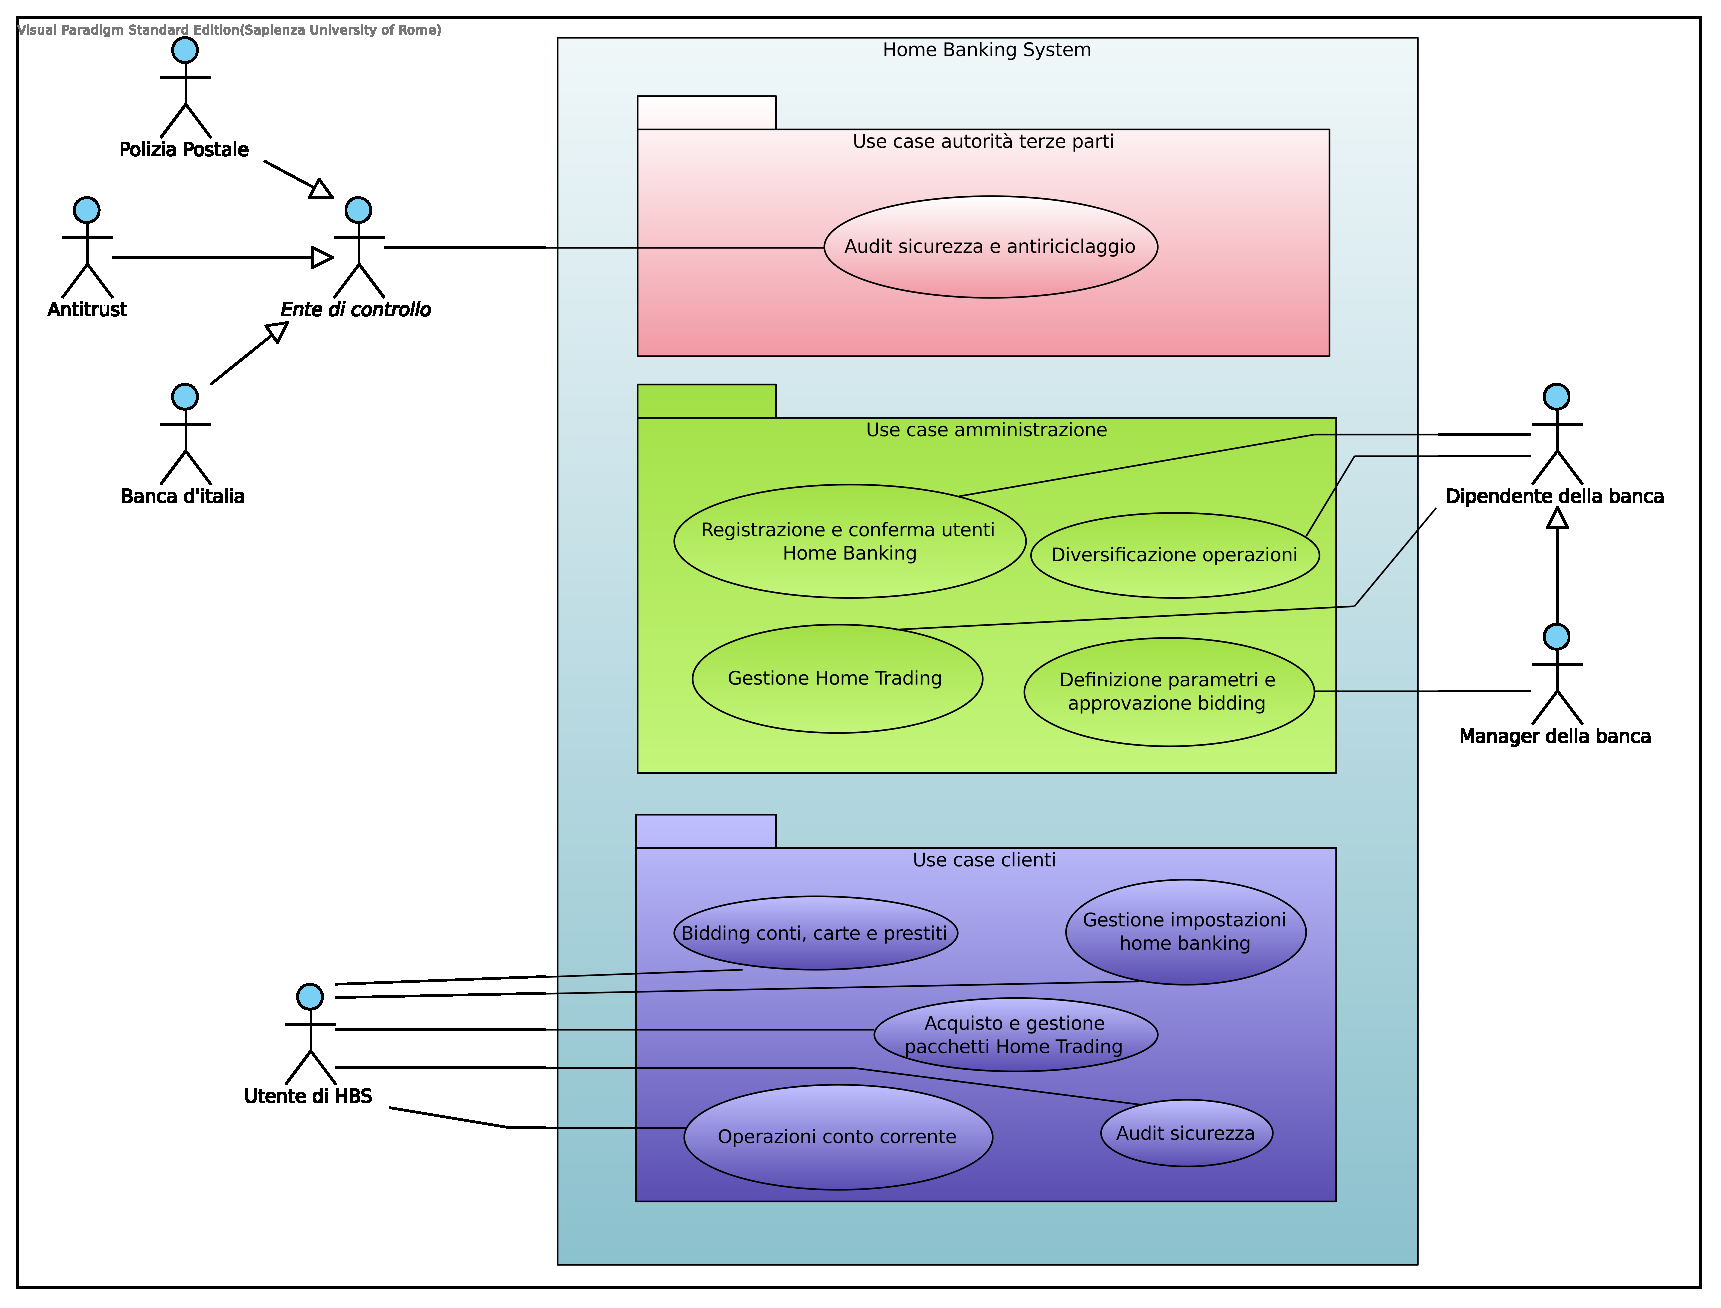
\includegraphics[width=\textwidth]{Images/Home_Banking_inception_use_cases.eps}
	\caption{Attori del sistema di Home Banking e relativi use cases.}
	\label{fig:use-cases}
\end{figure*}

\begin{figure*}
	\centering
	\includegraphics[width=\textwidth]{Images/use-cases/amministrazione-gestione-utenti.eps}
	\caption{Diagramma degli use case per la registrazione e gestione degli utenti da parte dell'amministrazione della banca.}
	\label{fig:use-cases:amministrazione:gestione-utenti}
\end{figure*}



\section{Specifica dei casi d'uso}

Di seguito \`e illustrata la specifica dei casi d'uso del sistema.

\subsection{\code{UC\_1} - Visualization Bidding }
\label{sec:use-case:BIDVIS}

\begin{ptable}{2}
\ptitle{Titolo}
\pcell{1}{
	Visualization Bidding (\code{UC\_BIDVIS\_1})
}
\pline
\ptitle{Descrizione use case}
\pcell{1}{
		I manager della banca possono ottenere delle \emph{visualization} delle regole di bidding realizzate. Una \emph{visualization} fornisce una rappresentaziona grafica intuitiva dell'insieme di bid approvati automaticamente, soggetti ad approvazione da parte di un manager, e respinti automaticamente.
}
\pline
\ptitle{Attori}
\pcell{1}{
		Manager della banca
}
\pline
\ptitle{Origine}
\pcell{1}{
		Requisiti funzionali e requisiti di usabilit\`a.
}
\pline
\ptitle{Pre-condizioni}
\pcell{1}{
		Almeno una regola di bidding \`e stata definita.
}
\pline
\ptitle{Flusso}
\pcell{1}{
		\begin{enumerate} \item Il manager seleziona una regola di bidding definita in HBS; \item il sistema di HBS realizza una \emph{visualization} della regola di bidding; \item la \emph{visualization} prodotta viene mostrata al manager nel browser. \end{enumerate}
}
\pline
\ptitle{Post-condizioni}
\pcell{1}{
		Nessuna
}
\pline
\ptitle{Side effects}
\pcell{1}{
		Nessuno
}
\end{ptable}

\subsection{\code{UC\_2} - Bidding Utente }
\label{sec:use-case:USRBID}

\begin{ptable}{2}
\ptitle{Titolo}
\pcell{1}{
	Bidding Utente (\code{UC\_USRBID\_2})
}
\pline
\ptitle{Descrizione use case}
\pcell{1}{
		Un utente di HBS pu\`o effettuare bid per conti correnti, carte di credito o prestiti.
}
\pline
\ptitle{Attori}
\pcell{1}{
		Utente di HBS
}
\pline
\ptitle{Origine}
\pcell{1}{
		Requisiti funzionali (requisito utente~\ref{req:itm:utente:funzionali:bidding:utente}, sez.~\ref{req:sec:utente:funzionali}, e requisito di sistema \idUSRBID).
}
\pline
\ptitle{Pre-condizioni}
\pcell{1}{
		Almeno una regola di bidding per l'oggetto richiesto (conto corrente, carta di credito o prestito) \`e stata definita..
}
\pline
\ptitle{Flusso}
\pcell{1}{
		\begin{enumerate} \item L'utente specifica i parametri del proprio bid;
\item l'utente invia il bid al sistema di HBS;
\item l'utente riceve un responso dal sistema di HBS riguardo l'approvazione, il rifiuto o la presa in carico del bid da parte del sistema stesso. \end{enumerate}
}
\pline
\ptitle{Post-condizioni}
\pcell{1}{
		Nessuna.
}
\pline
\ptitle{Side effects}
\pcell{1}{
		Se la proposta di bid \`e stata rifiutata, nessuno. Se la proposta di bid \`e stata accettata, il bid \`e stato memorizzato nel sistema come bid approvato automaticamente, e inviato a un dipendente della banca per la realizzazione. Se la proposta di bid \`e stata presa in carico per il controllo da parte di un manager della banca, la proposta di bid \`e stata inserita nel sistema come proposta non ancora approvata, ed \`e stata inviata al manager della banca.
}
\pline
\ptitle{Flusso alternativo}
\pcell{1}{
		In qualsiasi punto del workflow l'utente pu\`o interrompere l'inserimento della proposta di bid.
}
\pline
\ptitle{Post-condizioni alternative}
\pcell{1}{
		Nessuna.
}
\pline
\ptitle{Side effects alternativi}
\pcell{1}{
		Nessuno.
}
\end{ptable}

\subsection{\code{UC\_3} - Creazione Bidding }
\label{sec:use-case:CREABID}

\begin{ptable}{2}
\ptitle{Titolo}
\pcell{1}{
	Creazione Bidding (\code{UC\_CREABID\_3})
}
\pline
\ptitle{Descrizione use case}
\pcell{1}{
		Un manager della banca pu\`o creare una regola di bidding.
}
\pline
\ptitle{Attori}
\pcell{1}{
		Manager della banca.
}
\pline
\ptitle{Origine}
\pcell{1}{
		Requisiti funzionali (requisito di sistema \idCREABID).
}
\pline
\ptitle{Pre-condizioni}
\pcell{1}{
		Nessuna.
}
\pline
\ptitle{Flusso}
\pcell{1}{
		\begin{enumerate} \item Il manager seleziona una tipologia di bidding (carte di credito, conto corrente, prestito); \item \label{itm:uc:CREABID:parametro} il manager seleziona un parametro di scelta; \item il manager imposta i range di approvazione automatica, approvazione condizionata, e rifiuto automatico sul parametro scelto; \item opzionalmente, il manager torna al punto \ref{itm:uc:CREABID:parametro}; \item il manager inserisce la regola di bidding creata. \end{enumerate}
}
\pline
\ptitle{Post-condizioni}
\pcell{1}{
		Nessuna.
}
\pline
\ptitle{Side effects}
\pcell{1}{
		La regola di bidding realizzata \`e stata aggiunta al sistema di HBS.
}
\pline
\ptitle{Flusso alternativo}
\pcell{1}{
		In qualsiasi punto del workflow il manager pu\`o annullare l'operazione.
}
\pline
\ptitle{Post-condizioni alternative}
\pcell{1}{
		Nessuna.
}
\pline
\ptitle{Side effects alternativi}
\pcell{1}{
		Nessuno.
}
\end{ptable}





% \section{Corrispondenza casi d'uso / requisiti}

\newcommand{\vertical}[1]{\rotatebox[origin=c]{90}{#1}}
\newcommand{\V}{\checkmark}

Nella tabella \ref{table:tracking-requisiti} \`e illustrata la corrispondenza fra casi d'uso e requisiti funzionali del sistema.
Una spunta (\V) nella casella in riga $i$, colonna $j$, indica che il caso d'uso in riga $i$ realizza il requisito funzionale in colonna $j$.

%Magia: posso riferirmi al requisito \ref{req:itm:utente:funzionali:iscrizione}.
%Posso anche stampare l'id di un requisito, ad esempio \idLOGOP (o \shortidLOGOP in breve).

\begin{table}[h]
\resizebox{1\textwidth}{!}{\begin{minipage}{\textwidth}
\begin{center}
\begin{tabular}{r*{8}{|c}}
	& \vertical{\idSECAUTH}
	& \vertical{\idISCRCORR}
	& \vertical{\idLOGOP}
	& \vertical{\idCROPVEL}
	& \vertical{\idDISOPVEL}
	& \vertical{\idDISPAG}
	& \vertical{\idVERTIT}
	& \vertical{\idVERSAL} \\ \hline
	Prova &  & \checkmark & & \checkmark & & & & \\
\end{tabular}
\end{center}
\caption[Corrispondenza requisiti]{Corrispondenza fra requisiti e casi d'uso.}
\label{table:tracking-requisiti}
\end{minipage} }
\end{table}


\section{Registro modifiche}

\subsection{Elaboration}

\subsubsection{I iterazione}

Prima stesura documento.

\subsubsection{II iterazione}

Correzioni di errori.
Espanso use case model.
Aggiunto attore ``cliente della banca''.

\subsection{Construction}

\subsubsection{I iterazione}

Approfonditi use case principali.

%----------------------------------------------------------------------------------------
%	REFERENCE LIST
%----------------------------------------------------------------------------------------

%\nocite{banca_italia}
\printcustombib{}

%----------------------------------------------------------------------------------------
%	FIGURES
%----------------------------------------------------------------------------------------

\end{document}
